\section{Vorlesung 13 \href{https://tu-dresden.de/mn/math/algebra/das-institut/beschaeftigte/antje-noack/ressourcen/dateien/v120-1/MathMethInf13.pdf?lang=en}{(31.05.2019)}}
\begin{definition}[L-periodial]
	$f(x)$ heißt L-periodiel $(L>0)$, wenn gilt : $\forall \in \mathbf{R}: f(x+L)=f(x)$
\end{definition}
\begin{remark}
	Es genügt ,$2\pi$-perodiele Funktionen zu betrachten, denn 
\begin{align*}
f(x) \text{ L-perodial }\Rightarrow  g(x)&= f(x.\frac{L}{2\pi}) ist 2\pi\text{-perodiel, denn }\\
								g(x+2\pi)&= f((x+2\pi).\frac{L}{2\pi})= f(x.\frac{L}{2\pi}+L)=f(x\frac{L}{2\pi})=g(x)\\
f(x)  2\pi-periodiel \ \Rightarrow g(x)&= f(x\frac{2\pi}{L})\text{ ist L-Perodial}\\
\text{wir betrachten nur noch }& 2\pi-periodiele\text{ funktionen}
\end{align*}
\end{remark}
\begin{example}
	$\cos t$ ist $2\pi$-perodiel  
	$\underbrace{\cos(t\frac{2\pi}{\frac{2\pi}{k}})}_{cos(k.t)}$ ist 
	$\overset{\overset{\text{kleinste Periodenlänge}}{\downarrow}}{\frac{2\pi}{k}-}perodiel$ und auch 2$\pi$-perodiel\\
\begin{tikzpicture}
\begin{axis}[
height=5cm,
width=15cm,
axis y line = left,
axis x line = middle,
xticklabels = {$b$,$a$},
ytick       = \empty,
ymin = -2, ymax = 2,
  xmin=0,xmax=4*pi,
xlabel=$t$,
ylabel=$J$,
xtick={0,1.57,3.14,4.71,6.28},
xticklabels={$0$, ,,,$2\pi$}
]
\addplot[domain=0:4*pi,samples=200,blue] {cos(deg(x))}node[above,pos=0.97]{$\cos t$}; 
\end{axis}
\end{tikzpicture}
\end{example}
\begin{remark}
Die Funktionen $\cos(kt)$ und $\sin(kt)$ mit $k\in \{ 0,1,2,... \}   $ sind $2\pi$-periodiel\\ 
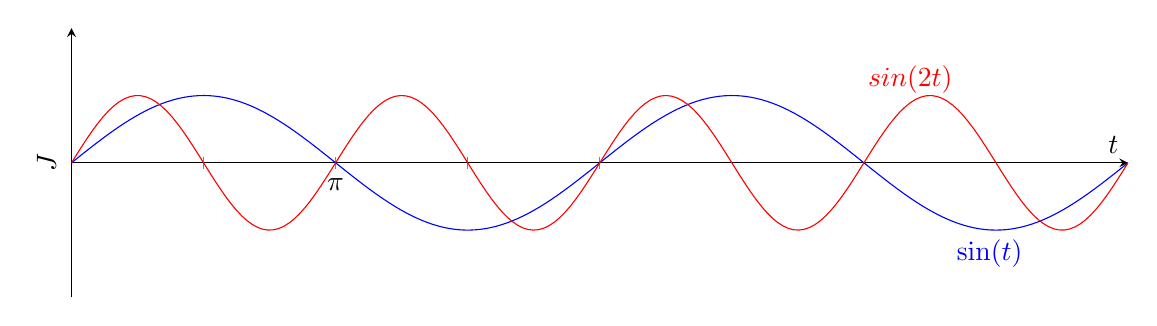
\begin{tikzpicture}
\begin{axis}[
height=5cm,
width=15cm,
axis y line = left,
axis x line = middle,
xticklabels = {$b$,$a$},
ytick       = \empty,
ymin = -2, ymax = 2,
xmin=0,xmax=4*pi,
xlabel=$t$,
ylabel=$J$,
xtick={0,1.57,3.14,4.71,6.28},
xticklabels={$0$, ,$\pi$,,}
]
\addplot[domain=0:4*pi,samples=200,blue] {sin(deg(x))}node[below,pos=0.87]{$\sin(t)$}; 
\addplot[domain=0:4*pi,samples=200,red] {sin(deg(2*x))}node[above,pos=0.80]{$sin(2t)$}; 
\end{axis}
\end{tikzpicture}
\end{remark}
\begin{remark}
$\underbrace{\frac{a_0}{2}.1+\sum_{k=1}^{n}(a_k.cos(k.t)+b_k.\sin(k.t))}_{\text{Trigonomisches Polynom der Ordnung nfalls} a_n \neq 0\text{ oder }b_n \neq 0}$
$a_k$, $b_k$ heißen FOURIER-koeffizienten
\end{remark}
 
	\begin{forest}
	[FOURIER-Theorie 
	[	kontinuierlich[Fourier-Reihen]  ]
	[Diskret [DFT] [FFT]]
	]
\end{forest}\\

\newpage
FOURIER-Synthese\\
gg: $a_k$, $b_k$\\
ges: Trigonometrisches Polynom\\
Fourier-Analyse\\
geg: $f(t)$\\
ges: $a_k$, $b_k$ so dass $f(t)$ (!unklar *udsinqieu**** durch ein Trigonometrisches Polynom und deren koff. betrachten werden kann)\\
\begin{remark}
$	C[0,2\pi,]$ ist der R-VR der auf $[0,2\pi]$ stetigen Funktionen \\

 \begin{align*}
f,g \in C[0,2\pi] \qquad f \neq g &: t \rightarrow f(t) + g(t)\\
r f &:t \rightarrow rf(t)  (!fehlt)\\
\underbrace{span( \{ 1,\cos t , \cos(2t),\dots,\sin t,\sin (2t),\dots   \}) }_{w}&\text{ ist ein UVR von }  C[0,2\pi]
\end{align*}
\textbf{gegeben:} 
\[ f(x) \in  C[0,2\pi] , 2\pi \quad periodisch   \]
\textbf{gesucht:} \[ f(x) \text{Bestapproximation von } f(x)  \text{ durch ein Element aus W. } \]  
\end{remark}
$\hat{f}(x)$ ist eine Orthogonal-Projektion von $f(x)$ in W. Dazu braucht man eine Orthogonal-Basis von W \\
z.z Die Elemente \{ 1 , cos(t) , cos(2t), ... , sin(t) , sin(2t), ... \} sind paarweise orthogonal.\\
\textbf{Behauptung}\\
Die Vektoren aus der oben erwähnten Mengen sind paarweise orthogonal bezüglich des Skalarprodukt.
Seien f , g stetige Funktionen aus $C[0,2 \pi]$  
\begin{align*}
\Rightarrow f \circ  g := \int_{0}^{2 \pi} {f(t) \times  g(t) dt } 
\end{align*}
Es gilt beispielsweise := $ cos(kt) \circ cos(ft)$
$$ = \int_{0}^{2 \pi} cos (kt) \times cos(ft)dt = \dots  $$
\begin{remark}
Sei $e^{i(x+y)}= e^{ix} \times e^{iy} $
\begin{align*}
cos(x+y) + i \times sin(x+y) &= (cos x + i \times sin x) 
(cos y + i \times sin y)\\
&= (cosx \times cos y - sin x \times sin y ) + i( \dots  )
\end{align*}
\end{remark}
\subsection{Additionstheoreme}
\begin{align*}
cos( x + y )&= cos x \times cos y - sin x \times sin y \\
cos( x \pm y ) &= cos x \times cos y \pm sin x \times sin \pm y \\
cos x \times cos y &= \frac{1}{2} (cos(x+y))+ cos (x-y)
\end{align*}
es geht weiter mit Beispiel
\begin{example}
\begin{align*}
&= \frac{1}{2} \int_{0}^{2 \pi} (cos(k+l)t + cos(k-l)t)dt\\
&= \frac{1}{2} \Big[ \frac{sin(k+l)t}{k+l} + \frac{sin(k-l)t}{k-l} \Big]_{0}^{2 \pi}\\
&= \frac{1}{2}(0 +0-0+0)=0
\end{align*}
\end{example}
\textbf{Die suche nach } $\hat{f}$
\begin{align*}
\hat{f}(t) &= \frac{f(t) \times 1}{1 \times}1 + \underbrace{\frac{f(t) cos(t)}{cos(t) \times cos(t)}cost }_{a_1} + \dots 
\\ &+ \underbrace{\frac{f(t) cos(2t)}{cos(2t) \times cos(2t)}}_{a_2} + \dots \\
&+ \underbrace{\frac{f(t) \times sin(t)}{sin(t) \times sin(t)}sin(t)}_{b_1} 
+ \underbrace{\frac{f(t) \times sin(2t)}{sin(2t) \times sin(2t)}sin(2t)}_{b_2} + \dots
\end{align*}
\subsection{Berechnung der Fourier-Koeffizienten : $a_k , b_k$}
\[ \Rightarrow a_k = \frac{f(t) \times cos(kt)}{cos(kt) \times cos(kt)} = \frac{1}{\pi} \int_{0}^{2 \pi} f(t) cos(kt) dt \quad k \geq 0 \]
\begin{remark}
\begin{align*}
\int_{0}^{2 \pi} (cos(kt))^2dt
\text{ Add Theorem } cos 2x &= (cos(x))^2-(sin(x))^2\\
&= (cos(x))^2 - (1 - cos(x))^2\\
&= 2(cos(x))^2 -1\\
&= \frac{1}{2} \int_{0}^{2 \pi} (1 + cos(2kt))dt\\
&= \frac{1}{2} \Big[ t + \frac{sin(2kt)}{2k} \Big ]_{0}^{2 \pi}\\
&= \frac{1}{2} [2 \pi - 0 - 0 + 0 ] = \pi
\end{align*}
\[ b_k = \frac{1}{n} \int_{0}^{2 \pi} f(t) \times sin (kt)dt \quad k \geq 1 \]
\textbf{Berechnung von $\hat{f}(t)$ wenn $k = 0$}
\begin{align*}
\hat{f}(t) = \frac{f(t) \times 1}{1 \times 1} \times 1 &= \frac{1}{\int_{1}^{2 \pi} 1 dt}\times \int_{0}^{2 \pi} f(t) \underbrace{cos (d.t)}_{1} dt\\
&= \frac{1}{2 \pi} \int_{0}^{2 \pi} f(t) cos (t)dt\\
&= \frac{1}{2} \times \frac{1}{2 \pi} \int_{0}^{2 \pi} f(t) cos (ot)dt
\end{align*}
\end{remark}
\begin{remark}
$$ \hat{f}(t) = \frac{a_0}{2} + \sum_{n}^{k=1} a_k cos(kt) + b_k sin (kt ) $$ heißt \textbf{Fourier Approximation} von f(x)
\end{remark}
\begin{theorem}
Sei $f(x) \in C[ 0 , 2 \pi]$ Dann existiert eine Fourier Reihe von $f(x)$
\end{theorem}
\begin{example}[von Sägezahnfunktion ]
% https://www.math.uni-hamburg.de/teaching/export/tuhh/cm/a2/07/vorl11_ana.pdf 
\begin{align*}
a_1 &= 1 \times f(t) = 2 \Big( \frac{sin(t)}{1} - \frac{sin(2t)}{2} + \frac{sin(3t)}{2}- \dots + \dots \Big)\\
t &= \frac{\pi}{2} \times f(\frac{\pi}{2}) = \frac{\pi}{2} = 2 \times 
\Big( \frac{sin(\frac{\pi}{2})}{1} -
\frac{sin(2 \frac{\pi}{2})}{2} +
\frac{sin(3 \frac{\pi}{2})}{3} - \dots + \dots \Big)\\
&= 2 \times \bigg( 1 - 0 - \frac{-1}{3} + 0 + \frac{1}{5} - \frac{1}{7} \bigg)\\
\frac{\pi}{4} &= \sum_{k = 1 }^{\infty} (-1)^{k+1}\frac{1}{k-1}\\
\frac{\pi}{2} &= 2 \sum_{k = 1 }^{\infty} (-1)^{k+1}\frac{1}{2k-1}
\end{align*}
\end{example}
